\documentclass{beamer}
% \usepackage{animate}
\usepackage{multimedia}
\usepackage[english,russian]{babel}

\usepackage{pgfpages}
\setbeameroption{show notes on second screen}
%https://tug.ctan.org/macros/latex/contrib/beamer/doc/beameruserguide.pdf

\usepackage[T2A]{fontenc}
\usepackage[utf8]{inputenc}

\setbeamertemplate{caption}[numbered]

\usetheme{CambridgeUS}
\usecolortheme{dolphin}

\title[ММК]{Метод Монте-Карло \\ Monte Carlo Method}
\author[Быковских Д.А.]{Быковских Дмитрий Александрович}
\date{07.12.2024}

\begin{document}
	\begin{frame}
		\titlepage
	\end{frame}
	%\section{Обзор}
	\begin{frame}{Содержание}
		\begin{itemize}
			\item 
			Определение, понятия, история
			\item
			Генератор псевдослучайных чисел
			\item
			Пример
			\item
			Квази МКМ
			\item 
			Скорость сходимости
			\item 
			Применение метода в компьютерной графике
			\item
			MISER algorithm
		\end{itemize}

		\note{
			% Схема анализа задачи
			% 	\begin{enumerate}
			% 		\item
			% 		Постановка проблемы/задачи.
			% 		\item
			% 		Создание модели.
			% 		\item
			% 		Общий алгоритм.
			% 		\item
			% 		Случайная величина.
			% 		\item
			% 		Точность.
					
			% 		когда знаешь, точный результат
					
			% 		когда не знаешь, точный результат
			% 		\item
			% 		Погрешность.
			% 		\item
			% 		Как уменьшить погрешность?
			% 	\end{enumerate}
			
		}
	\end{frame}
	\begin{frame}{Краткая справка}{Monte-Carlo Method (MCM)}
		Монте-Карло метод (ММК) --- численный метод решения математических задач при помощи моделирования случайных величин.
		%Ссылка на Соболь Монте-Карло Метод Популярные лекциии по математике
		
		Название происходит от города Монте-Карло в княжестве Монако, знаменитого своим игорным домом. 
		
		\note{Рулетка --- простейший прибор получения случайной величины. }
		
		Датой рождения считается 1949 г., когда появилась статья под названием \href{https://web.williams.edu/Mathematics/sjmiller/public_html/105Sp10/handouts/MetropolisUlam_TheMonteCarloMethod.pdf}{The Monte Carlo Method (Н.~Метрополис и С.~Улам)}.
		
		Теоретическая основа известна давно.
		
		\note{ \footnotesize
			
		Метод Монте-Карло — [84; 85].
		
		Первая работа по использованию вероятностного метода была опубликована А. Холлом в 1873 году именно при организации стохастического процесса экспериментального определения числа $\pi$ путем бросания иглы на лист линованной бумаги. Идея такого эксперимента возникла у Ж.Л.Л. Бюффона для
		вычисления числа $\pi$ в 1777 году.
				
		Бурное развитие и применение методов статистического моделирования (Монте-Карло) в различных областях прикладной математики началось с середины прошлого столетия. Это было связано с решением качественно новых задач, возникших при исследовании новых процессов. 
		
		Одним из первых, кто применил ММК для моделирования траекторий нейтронов был Дж. фон Нейман. 
		
		Первая работа с систематическим изложением была опубликована в 1949 году Н.К. Метрополисом и С.М. Уламом. 
		Метод Монте-Карло применялся для решения линейных интегральных уравнений, в котором решалась задача о прохождении нейтронов через вещество.
		
		% 1. Hall, A. On an experiment determination of π / A. Hall // Messeng. Math. –– 1873. –– No. 2. –– P. 113––114. 108
		% 2. Metropolis, N. The Monte-Carlo method / N. Metropolis, S. Ulam // J. Amer. Stat. Assoc. –– 1949. –– Vol. 44, no. 247. –– P. 335––341.
		% 3. Соболь, И. М. Численные методы Монте-Карло / И. М. Соболь. –– М. : НАУКА, 1973. –– 312 с.
		% 4. Марчук, Г. И. Метод Монте-Карло в атмосферной оптике / Г. И. Марчук, Г. А. Михайлов. –– М. : Наука, 1976. –– 145 с.
	}
	
 	\end{frame}
	\begin{frame}{Краткая справка}
		Особенности метода:
		\begin{enumerate}
			\item 
			Простая структура вычислительного алгоритма, т.е. необходимо описать действие одного шага.
			А потом множество шагов усреднить.
			Метод статистических испытаний.
			\item
			Ошибка вычислений, как правило, пропорциональная 
			$$\sqrt{\frac{D}{N}},$$ 
			где $D$ --- некоторая постоянная, а $N$ --- число испытаний.
			%проанализировать это.
			Метод эффективен, когда высокая точность не сильно важна.
			
		\end{enumerate}
		
		Задачи решаемые с помощью ММК:
		\begin{enumerate}
			\item
			Любой процесс, на протекание которого влияют случайные факторы.
			\item 
			Для любой задачи можно искусственно придумать вероятностную модель или даже несколько.
		\end{enumerate}		
	\end{frame}

	\begin{frame}{Случайные числа}
		Случайная величина --- математический объект, которая представляет собой функцию, сопоставляющая каждому элементарному исходу случайного эксперимента числовое значение.

		Функция распределения случайной величины предоставляет информацию о том, как вероятность распределена между различными значениями случайной величины. В теории вероятностей часто используются различные распределения (например, равномерное, биномиальное, нормальное), чтобы моделировать различные типы случайных величин.
		
		Генератор псевдослучайных чисел (ГПСЧ) --- алгоритм или устройство, создающее последовательность чисел, которые кажутся случайными, но на самом деле образуют детерминированную последовательность. Эти числа обычно используются в компьютерных программах для имитации случайности в различных приложениях, таких как моделирование, шифрование, игры и другие.

		\note{
Случайные величины могут быть классифицированы как
\begin{enumerate}
	\item 
	Дискретная случайная величина.\\
			Принимает конечное или счетное множество значений.\\
			Вероятности каждого значения определены явно.
	\item
	Непрерывная случайная величина.\\
			Принимает значения из непрерывного интервала.\\
			Вероятность любого конкретного значения равна нулю (в отличие от дискретных случайных величин).
			Определяется функцией плотности вероятности (например, нормальное распределение).
\end{enumerate}

	Случайные величины также могут быть классифицированы как одномерные (включающие только одну переменную) или многомерные (включающие несколько переменных). Многомерные случайные величины используются, например, в многомерных статистиках и теории случайных процессов.
	
}

	\end{frame}

	% \begin{frame}{Вычисление площади фигуры}{Пример}
	% 	\note{Стрелок плохо стрелят или хорошо, как это скажется на результатах?}
	% \end{frame}
	
	\begin{frame}{Вычисление площади определенного интеграла}{Пример}
		Постановка задачи
		\[
		I = \int_{a}^{b} f(x) dx
		\]
		
		Метод центральных прямоугольников
		\[
		I 
		\approx 
		\sum_{i=1}^{N} f(x_i) \Delta x_i 
		=
		\frac{b-a}{N} \sum_{i=1}^{N} f(x_i)
		,
		\]
		где $\sum_{i=1}^{N} \Delta x_i = b - a$.
		\[
		I
		=
		(b - a) M [f(x)]
		\]
		Пусть плотность распределения $\rho(x) = \frac{1}{b-a}$. Тогда интеграл можно вычислить следующим образом:
		\[
		I
		= 
		\int_{a}^{b} \frac{f(x)}{\rho(x)} \rho(x) dx
		= 
		M \Bigg[\frac{f(x)}{\rho(x)}\Bigg] 
		\approx
		\frac{1}{N} \sum_{i=1}^{N} \frac{f(\xi_i)}{\rho(\xi_i)}
		.
		\]
		\note{Estimator --- правило для вычисления статистической оценки, определяющее скорость сходимости.
		% $\xi_i$ --- описать.

			\begin{figure} 
				% http://aco.ifmo.ru/el_books/numerical_methods/lectures/glava2_2.html
				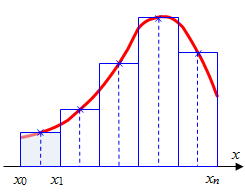
\includegraphics[width=0.47\textwidth]{images/glava2_clip_image_p001.png}
				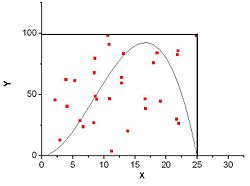
\includegraphics[width=0.5\textwidth]{images/mc_integration.jpg}
				\caption{Метод центральных прямоугольников (слева) и метод Монте-Карло (справа)}
			\end{figure}
		
		}
	\end{frame}

	\begin{frame} {Оценка погрешностей при моделировании независимых испытаний}

		
		Пусть $\xi=\xi(\omega)$ --- интегрируемая случайная величина, тогда математическое ожидание $M\xi$ и дисперсия $D\xi$ случайной величины $\xi$ определяется формулами:
		\[
			% \begin{equation} 
			M\xi = \int\limits_{\varOmega} \xi (\omega) P(\mu (d \omega) )
			= \int \limits_{R_1} x  d F_{\xi}(x) 
			,
			% \end{equation} 
		\]
		где $P(\mu( d \omega))$ %= P(\omega) d\omega$ 
		--- вероятность того, что величина $\omega$ определена на интервале $d\omega$, 
		$F_{\xi} (x)=\int \limits_{-\infty}^{x} f_{\xi} (t) \mu (dt)$ --- функция распределения случайной величины $\xi$ в точке $x$.
		\[
			% \begin{equation} 
			D\xi = \int \limits_{R_1} {[x - M \xi]}^2 d F_{\xi}(x) 
			= M \xi^2 - {(M \xi)}^2
			% \end{equation} 
		\]

				
		\note{
			% Одно из главных преимуществ стохастических расчетных методов связано с тем, что можно оценить статистическую ошибку, т.е. в ходе расчета можно вычислить не только средние значения, но и дисперсию.
			%Погрешность полученных статистических оценок макроскопических параметров (далее макроскопические параметры) можно оценить следующими способами.

			Для дискретной случайной величины \(\xi\), принимающей значения \(x_1, x_2, \dots, x_n\) с вероятностями \(p_1, p_2, \dots, p_n\), формулы для математического ожидания ($M\xi$) и дисперсии ($D\xi$) запишутся следующим образом:

			% Математическое ожидание
			
			\[
				M\xi 
				\approx
				\sum_{i=1}^N x_i p_i
			\]
			
			% Дисперсия

			\[
				D\xi 
				\approx
				\sum_{i=1}^N (x_i - \sum_{i=1}^N x_i p_i)^2 p_i = \sum_{i=1}^N x_i^2 p_i - \Big(\sum_{i=1}^N x_i p_i\Big)^2
			\]

		}
	\end{frame}

	\begin{frame} {Оценка погрешностей при моделировании независимых испытаний}
		%\textit{Частный случай центральной предельной теоремы.}
		Доверительный интервал $(M\xi - \delta, M\xi + \delta)$, в котором находится истинное значение $M\xi$ случайной величины $\xi$ %,распределенной по нормальному закону, 
		с заданной вероятностью~$P$, определяется следующим образом:
		\[
			% \begin{equation}
			P \left\{ \left| \frac{1}{n} \sum^n_{i=1} \xi_i - M\xi \right| 
			\leqslant  \frac{\alpha \sigma}{\sqrt{n}} \right\} 
			= 2 \varPhi(\alpha) 
			,
			% \end{equation}
		\]
		где 
		% $\hat{\mu}$ --- математическое ожидание $M \xi$; \linebreak
		$\xi_i$ --- неизвестная величина, полученная в результате $i$-го испытания; 
		$n$ --- независимые истории (число испытаний); 
		$\sigma = \sqrt{D \xi}$~---~среднеквадратичное отклонение; %погрешность, зависящая от числа испытаний. 
		$\varPhi (\alpha)= \frac{1}{2 \sqrt{\pi}}  \int \limits_{0}^{\alpha}  e^{-t^2} dt $~---~функция Лапласа.

		\note{
			Правило трех сигм.

			Доверительный интервал $(M\xi - 3\sigma, M\xi + 3\sigma)$, в котором находится истинное значение $M\xi$ случайной величины $\xi$, распределенной по нормальному закону, с заданной вероятностью~$P$, определяется следующим образом
			\[
				P \left\{ \left| \frac{1}{n} \sum^n_{i=1} \xi_i - M\xi\right| 
				\leqslant  \frac{3 \sigma}{\sqrt{n}} \right\} 
				\approx 0.9973
				,
			\]
		}
	
	\end{frame}
	
	\begin{frame}{Физически-корректный рендеринг}{Physically-Based Rendering}
		
		Физически-корректный рендеринг (Physically Based Rendering, PBR) --- подход к генерации изображений, который стремится моделировать физические свойства света и материалов для достижения более реалистичных результатов.

		\[
			L_o(x, \omega_o) =
			\int_{\Omega} \bigg( 
			k_d \frac{c}{\pi} 
			+
			k_s \frac{DFG}{4 (\omega_o \cdot n) (\omega_i \cdot n)} 
			\bigg)
			L_i(x,\omega_i) (n \cdot \omega_i)
			d \omega_i
		\]

		\note {
			\footnotesize
			Основные принципы физически-корректного рендеринга включают в себя:

			\begin{itemize}
				\item 
				Моделирование света.
				Учет различных источников света, их цветовых температур, направления и интенсивности.
				Учет закона сохранения энергии в процессе отражения и преломления света.
				\item 
				Моделирование материалов.
				Физически-корректные модели отражения, преломления и поглощения света в зависимости от типа материала.
				\item 
				Моделирование теней и окружающей среды.
				Учет влияния теней от различных объектов и источников света.
				Моделирование окружающей среды для более точного воссоздания условий освещения.
				\item 
				Многоканальные текстуры.
				Использование текстур с несколькими каналами для более точного представления различных характеристик материалов, таких как шероховатость, металлические свойства и др.
				\item 
				Моделирование камеры.
				Учет характеристик камеры, таких как диафрагма и выдержка, для более реалистичного эффекта глубины резкости и затемнения по краям кадра.
			\end{itemize}

		}

	\end{frame}

	
	\begin{frame}{Вычисление энергетической яркости}

		Формулы энергетической яркости поверхности в конкретном направлении
		% \[
		% 	I = \frac{\Phi}{d \omega}
		% \] 
		\[
			L = \frac{d^2 \Phi}{\cos \theta d \omega d A}
		\] 
		\[
			L \cos \theta d \omega = \frac{d^2 \Phi}{ d A}
		\] 
		где 
		$L$ --- энергетическая яркость (Radiance), описывает количество светового потока, излучаемого поверхностью в определенном направлении, на единичную площадку и в единичный угловой диапазон ($W/(m²\cdot sr)$);
		$d^2 \Phi$ --- элемент светового потока (Flux) через малую площадку $dA$  в малом угловом диапазоне $d \omega$;
		$\cos \theta$ --- косинус угла между нормалью к поверхности и направлением, в котором измеряется энергетическая яркость;
		$dA$ --- элемент площади поверхности, через которую измеряется световой поток;
		$d \omega$ --- элемент углового диапазона, в пределах которого измеряется световой поток.
		
		\note{
			\begin{figure} 
				% http://www.codinglabs.net/article_physically_based_rendering.aspx
				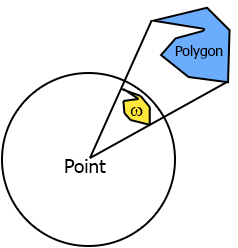
\includegraphics[width=0.48\textwidth]{images/solid_angle.png}
				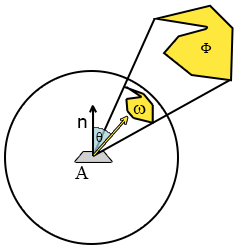
\includegraphics[width=0.48\textwidth]{images/radiance.png}
				\caption{Схема расчета телесного угла и энергетической яркости}
			\end{figure}
		}
	\end{frame}
	
	\begin{frame}{Вычисление площади единичной полусферы}
		Площадь единичной полусферы
		\[
			S_\text{hemisphere} 
			= 
			\int_{\Omega_+} d \omega 
			= 
			\int_{0}^{2\pi}\int_{0}^{\pi / 2} \sin \theta  d \theta d \phi
			= 
			\int_{0}^{\pi / 2} \sin \theta d \theta \int_{0}^{2\pi} d \phi
			=
			2 \pi
		\]


		Расчетная формула
		\[
			S_\text{hemisphere} 
			\approx
			\frac{\pi}{2 N_1}
			\frac{2 \pi}{N_2}
			\sum_{j=1}^{N_2} \sum_{i=1}^{N_1}
			\sin(\theta_i)
			=
			\sum_{j=1}^{N_2} \sum_{i=1}^{N_1}
			\sin(\theta_i) \Delta \theta_i \Delta \phi_j
			=
			\sum_{j=1}^{N_2} \sum_{i=1}^{N_1} \Delta S_{ij}
			,
		\]
		где 
		$\sum_{i=1}^{N_1} \Delta \theta_i = \pi /2$;
		$\sum_{j=1}^{N_2} \Delta \phi_j = 2 \pi$.

		\vspace{0.5cm}
		\footnotesize
		Примечание.\\
		Есть более удобный способ расчета.


		\note{
			\begin{figure} 
				% https://habr.com/ru/articles/426987/
				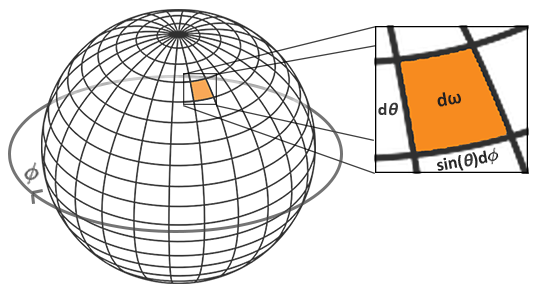
\includegraphics[width=0.9\textwidth]{images/sphere_scheme.png}
				\caption{Иллюстрация к интегрированию в сферической системе координат}
			\end{figure}
		}
	\end{frame}

	\if 0
	%Объединить и переписать

	\begin{frame}{Вычисление диффузного рассеивания}
		Площадь единичной полусферы
		\[
			L_o(x,\phi_o,\theta_o) 
			= 
			k_d \frac{c}{\pi}
			\int_{\Omega_+} () d \omega 
			= 
			\int_{0}^{2\pi}\int_{0}^{\pi / 2} \sin \theta  d \theta d \phi
			= 
			\int_{0}^{\pi / 2} \sin \theta d \theta \int_{0}^{2\pi} d \phi
			=
			2 \pi
		\]

		Расчетная формула

		\[
			S_\text{hemisphere} 
			\approx
			\frac{\pi}{2 N_1}
			\frac{2 \pi}{N_2}
			\sum_{j=1}^{N_2} \sum_{i=1}^{N_1}
			\sin(\theta_i)
			=
			\sum_{j=1}^{N_2} \sum_{i=1}^{N_1}
			\sin(\theta_i) \Delta \theta_i \Delta \phi_j
			,
		\]
		где 
		$\sum_{i=1}^{N_1} \Delta \theta_i = \pi /2$;
		$\sum_{j=1}^{N_2} \Delta \phi_j = 2 \pi$.

		\note{
			\begin{figure} 
				% https://habr.com/ru/articles/426987/
				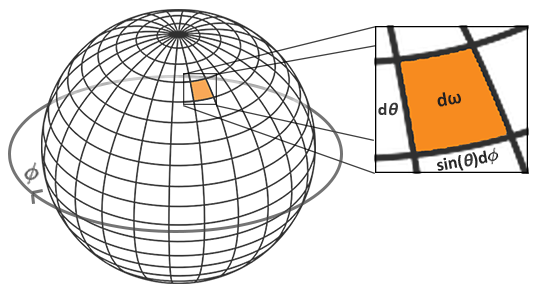
\includegraphics[width=0.95\textwidth]{images/sphere_scheme.png}
				\caption{Иллюстрация к интегрированию в сферической системе координат}
			\end{figure}
		}
	\end{frame}

	\begin{frame}{Вычисление диффузного рассеивания}
		Первая формула представляет собой уравнение отраженной энергетической яркости $L_o$ в точке $p$ на поверхности, ориентированной в направлении с углами $\phi_o$ и $\theta_o$.

		\[
			L_o(p,\phi_o,\theta_o) = k_d \frac{c}{\pi}
			\int_{\phi=0}^{2\pi} \int_{\theta=0}^{\pi / 2}
			L_i(p, \phi_i, \theta_i) \cos(\theta) \sin(\theta) d\phi d\theta
		\]			
			% Вторая формула представляет ту же отраженную излучательную способность, но в дискретной форме, используя суммирование по дискретным угловым интервалам $ϕ$ и $θ$. Параметры $N1$ и $N2$ определяют количество дискретных угловых шагов в соответствующих направлениях, а $kd$- коэффициент диффузного отражения, $c$ - коэффициент яркости.
			Формула расчета отраженной энергетической яркости
	\[
		L_o(p,\phi_o,\theta_o) \approx k_d \frac{c }{\pi} %\frac{1}{N_1 N_2}
		\sum_{j=0}^{N_1} \sum_{k=0}^{N_2}
		L_i(p, \phi_i, \theta_i) \cos(\theta_k) \sin(\theta_k) \Delta \phi_j \Delta \theta_k
	\]
		\note{
			\begin{figure} 
				% https://habr.com/ru/articles/426987/
				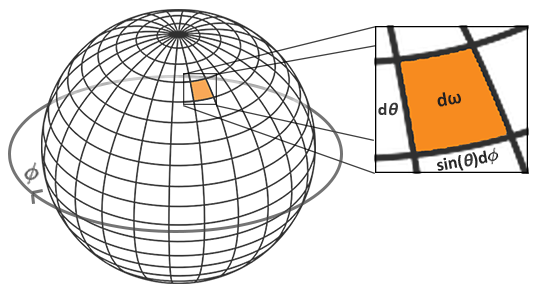
\includegraphics[width=0.95\textwidth]{images/sphere_scheme.png}
				\caption{Иллюстрация к интегрированию в сферической системе координат}
			\end{figure}
		}
	\end{frame}

	\fi
	
	\begin{frame}{Вычисление диффузного рассеивания}
		Рассмотрим следующее выражение
		\[
			L_o(x,\omega_o) = k_d \frac{c}{\pi}
			\int_{\Omega}
			L_i(x, \omega_i) (n \cdot \omega_i) d \omega_i
		\]

		Его расчетная формула будет иметь вид
		\[
			L_o(x,\omega_o) 
			\approx 
			k_d \frac{c}{\pi} \frac{1}{N}
			\sum_{i = 1}^{N}
			L_i(x, \omega_i) (n \cdot \omega_i)
			=
			k_d \frac{c}{\pi}
			\sum_{i = 1}^{N}
			L_i(x, \omega_i) (n \cdot \omega_i) \Delta \omega_i
		,
		\]
		где 
		$\omega_i$ --- входящий вектор направления рассчитывается случайным образом с равномерным законом распределения.


		\note{
			\begin{figure} 
				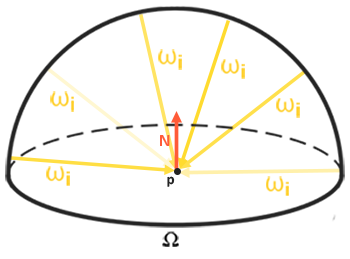
\includegraphics[width=0.65\textwidth]{images/w_i_and_omega.png}
				\caption{Иллюстрация усредненной суммы энергетической яркости внутри полусферы}
			\end{figure}
		}
	\end{frame}


	\begin{frame}{Квази-метод Монте-Карло}{Quasi-Monte Carlo Method}
		
		Квази-метод Монте-Карло представляет собой вариацию метода Монте-Карло, который использует квазислучайные последовательности вместо полностью случайных чисел. В отличие от стандартных случайных чисел, квазислучайные последовательности обладают определенными детерминированными свойствами, направленными на создание последовательности чисел, которые стремятся к равномерному покрытию пространства.

		Основная идея квази-метода Монте-Карло состоит в том, чтобы заменить случайные числа последовательностью чисел с некоторыми хорошими свойствами равномерного распределения. Эти последовательности разрабатываются так, чтобы минимизировать дисперсию оценок интегралов, т.е. улучшить скорость сходимость метода, и обеспечивать равномерное покрытие пространства.
		
		

		% Существует несколько способов создания случайных выборок. 
		% По умолчанию каждая точка выборки полностью случайна. Однако, используя свойства квазислучайных последовательностей, можно создавать наборы векторов с интересными свойствами. 
		% Например, при создании выборок для процесса интегрирования можно применять последовательности низкого несоответствия. Эти последовательности обеспечивают случайность точек выборки, но в целом они равномерно распределены, что полезно для интеграции.

		% Использование последовательностей низкого несоответствия при создании выборок для интеграции называется квази-методом Монте-Карло. Эти методы сходятся быстрее, что важно для производительных приложений.
		
		% Дополнительно, выборка по значимости ускоряет сходимость. Например, для зеркальных отражений важно сфокусировать генерацию векторов выборки в области зеркального лепестка с использованием смещенной функции оценки для метода Монте-Карло. Такие векторы выборки вне зеркального лепестка не влияют на интегральное выражение зеркальной компоненты и могут быть проигнорированы, что улучшает эффективность процесса.
		% https://math.spbu.ru/ru/mmeh/AspDok/pub/2009/Rukavishnikova.pdf
		\note{
			\begin{figure} 
				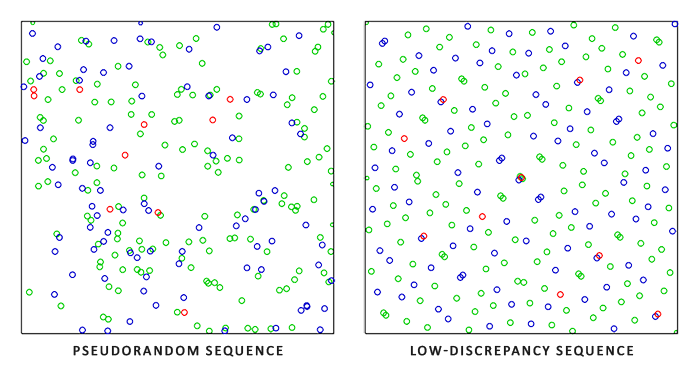
\includegraphics[width=0.9\textwidth]{images/quasi_monte_carlo_example.png}
				\caption{Результаты моделирования: псевдослучайная последовательность (слева) и последовательность низкого несоответствия (справа)}
			\end{figure}
		}
	\end{frame}

	\begin{frame}{MISER algorithm}
		MISER algorithm позволяет адаптивно распределять вычислительные ресурсы в зависимости от сложности функции на различных участках интервала интегрирования. Это улучшает эффективность численного интегрирования, особенно для функций с различной степенью изменчивости.
		% Этот метод часто используется для вычисления определенных интегралов.

		Описание метода

		\begin{enumerate}
			\item
			Задание начального интервала интегрирования.
			\item 
			Разбиение текущего интервала на более мелкие подинтервалы.
			\item 
			Вычисление приближенных значений на каждом подинтервале.
			\item 
			Оценка погрешности.
			\item 
			Адаптация разбиения за счет увеличения количества подинтервалов в областях с большой погрешностью.
			\item 
			Повторение процесса (шагов 3-5) до достижения заданной точности.
		\end{enumerate}

\note{
	\begin{figure} 
		% https://www.maxwellrules.com/math/montecarlo_integration.html
		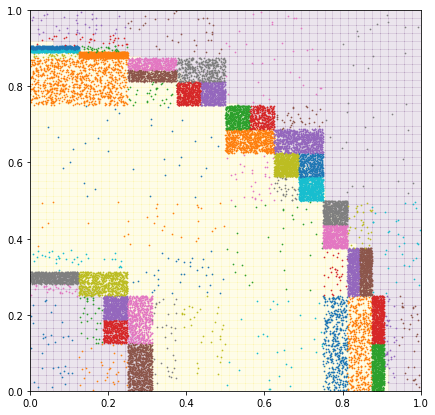
\includegraphics[width=0.55\textwidth]{images/miser_donut.png}
		\caption{Результат моделирования методом MISER при вычислении интеграла}
	\end{figure}

}

	\end{frame}

	\begin{frame}{Заключение}
		Литература
		\begin{enumerate}
			\item \href{https://math.ru/lib/plm/46}{Соболь И.М. Метод Монте-Карло (Популярные лекциии по математике, выпуск 46)}
			\item \href{http://aco.ifmo.ru/el_books/numerical_methods/lectures/glava2_2.html}{Учебное пособие по курсу "Численные методы в оптике"}
			\item \href{http://www.codinglabs.net/article_physically_based_rendering.aspx}{Coding Labs --- Physically Based Rendering}
			\item \href{https://www.maxwellrules.com/math/montecarlo_integration.html}{Maxwell rules --- Monte Carlo Integration}
			\item \href{https://habr.com/ru/articles/426987/}{Learn OpenGL. Урок 6.3 --- Image Based Lighting. Диффузная облученность}
		\end{enumerate}

	\end{frame}
	
\end{document}